\begin{frame}
	\Huge Tiefensuche
	\Large depth-first search, BFS
\end{frame}

\begin{frame}
	\frametitle{Tiefensuche}
	\framesubtitle{Einführung}
	\begin{KITexampleblock}{Indiana Jones and the Fate of Atlantis}
		Indiana Jones braucht unsere Hilfe! Er ist auf der Suche nach einer mysteriösen Statue muss er ein Labyrinth überwinden. Alles was er als Hilfsmittel besitzt ist eine (unendlich lange )rote Schnur. Wie geht Indy vor, um möglichst wenig Zeit zu verschwenden?	
	\end{KITexampleblock}
		\pause 
		\bigskip	
	\heading{Anforderungen}
	\begin{itemize}
		\item findet stets die Lösung, wenn sie existiert
		\item vermeidet doppelte Wege
	\end{itemize}
\end{frame}

\begin{frame}
	\frametitle{Tiefensuche}
	\framesubtitle{Einführung}
	\heading{Strategie}
	\begin{itemize}
		\item Die ganze Zeit lang spannen wir unsere rote Schnur und markieren damit bereits gesehene Wege.
		\item Wenn wir auf eine Gabelung stoßen, gehen wir immer einen Weg, den wir noch nicht gesehen haben.
		\item Wenn wir auf eine Sackgasse stoßen, gehen wir zurück zu der letzten Gabelung, in der sich noch ein ungesehener Weg befindet.
	\end{itemize}
\end{frame}

\begin{frame}
	\frametitle{Tiefensuche}
	\framesubtitle{Einführung}
	\begin{center}
	\includegraphics<1-1>{labyrinth01.eps}
	\includegraphics<2-2>{labyrinth02.eps}
	\includegraphics<3-3>{labyrinth03.eps}
	\includegraphics<4-4>{labyrinth04.eps}
	\includegraphics<5-5>{labyrinth05.eps}
	\includegraphics<6-6>{labyrinth06.eps}
	\includegraphics<7-7>{labyrinth13.eps}
\end{center}
\end{frame}

\begin{frame}
	\frametitle{Tiefensuche}
	\framesubtitle{rekursive Implementierung}
	\lstset{basicstyle=\scriptsize, commentstyle=\color{mygreen},frame=single}
	\lstinputlisting[language=C++,firstline=5, lastline=21]{sourcecode/dfs.cpp}
\end{frame}

\begin{frame}
	\frametitle{Tiefensuche}
	\framesubtitle{graphische Darstellung}
	\begin{center}
		\includegraphics[scale = 0.4]<1-1>{graph01.eps}
		\includegraphics[scale = 0.4]<2-2>{graph02.eps}
		\includegraphics[scale = 0.4]<3-3>{graph03.eps}
		\includegraphics[scale = 0.4]<4-4>{graph04.eps}
		\includegraphics[scale = 0.4]<5-5>{graph05.eps}
		\includegraphics[scale = 0.4]<6-6>{graph06.eps}
		\includegraphics[scale = 0.4]<7-7>{graph07.eps}
		\includegraphics[scale = 0.4]<8-8>{graph08.eps}
		\includegraphics[scale = 0.4]<9-9>{graph09.eps}
		\includegraphics[scale = 0.4]<10-10>{graph10.eps}
		\includegraphics[scale = 0.4]<11-11>{graph11.eps}
		\includegraphics[scale = 0.4]<12-12>{graph12.eps}
		\includegraphics[scale = 0.4]<13-13>{graph13.eps}
		\includegraphics[scale = 0.4]<14-14>{graph14.eps}
		\includegraphics[scale = 0.4]<15-15>{graph15.eps}
		\includegraphics[scale = 0.4]<16-16>{graph16.eps}
		\includegraphics[scale = 0.4]<17-17>{graph17.eps}
		\includegraphics[scale = 0.4]<18-18>{graph18.eps}
		\includegraphics[scale = 0.4]<19-19>{graph19.eps}
		\includegraphics[scale = 0.4]<20-20>{graph20.eps}
			\end{center}
\end{frame}

\begin{frame}
	\frametitle{Tiefensuche}
	\framesubtitle{informell}
	\begin{itemize}
		\item Laufzeit: $\mathcal{O}(|V| + |E|)$, wenn der Graph als Adjazenzliste gespeichert ist oder als Adjazentmatrix $\mathcal{O}(|V|^2)$
		\item Die Tiefensuche ist nicht optimal, wird im Allgemeinen nicht die kürzeste Verbindung zum Ziel gefunden.
		\item Der Speicherbrauch ist linear, da nur Informationen darüber gespeichert werden, ob ein Knoten schon besucht wurde.
	\end{itemize}
\end{frame}

\begin{frame}
		\frametitle{Tiefensuche}
		\framesubtitle{mögliche Probleme}
		\begin{itemize}
			\item Der Graph ist unendlich groß, in diesem Fall gibt es keine Möglichkeit, für jeden Knoten Informationen zu speichern.
			\item Es ist nach einem optimalen Ergebnis gefragt.
			\item Durch die vielen Rekursionsebenen wird das Rekursionslimit vom Betriebssystem überschritten.
		\end{itemize}
\end{frame}

\begin{frame}
	\frametitle{Tiefensuche}
	\framesubtitle{nichtrekursive Implementierung}
	\lstset{basicstyle=\scriptsize, commentstyle=\color{mygreen},frame=single}
	\lstinputlisting[language=C++,firstline=14, lastline=28]{sourcecode/nrdfs.cpp}
\end{frame}

\begin{frame}
	\frametitle{Tiefensuche}
	\framesubtitle{nichtrekursive Implementierung}
	\lstset{basicstyle=\scriptsize, commentstyle=\color{mygreen},frame=single}
	\lstinputlisting[language=C++,firstline=29, lastline=39]{sourcecode/nrdfs.cpp}
\end{frame}

\begin{frame}
	\frametitle{Tiefensuche}
	\framesubtitle{Beispielproblem}
	\begin{KITinfoblock}{Dominator}
		Ein Knoten X eines Graphen dominiert einen anderen Knoten Y, wenn alle Wege von einem gegebenen Startknoten zu Y durch X gehen müssen. Wenn ein Knoten Z nicht vom Startknoten erreicht werden kann, hat Z keinen Dominator.
	\end{KITinfoblock}
	\begin{center}
			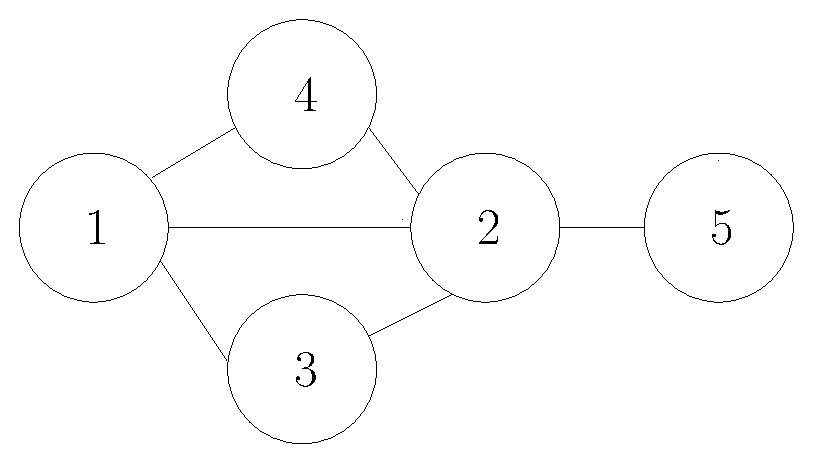
\includegraphics[scale = 0.6]{dominator}
	\end{center}
\end{frame}

\begin{frame}
	\frametitle{Tiefensuche}
	\framesubtitle{Beispielproblem}
		\begin{KITexampleblock}{Dominator}
			Gegeben sei ein Graph. Die Aufgabe ist es, für einen gegebenen Graphen für jeden Knoten die Dominator auszurechnen. Dabei ist zu erwähnen, dass der Eingabegraph sehr klein sind, mit weniger als 100 Knoten.
		\end{KITexampleblock}
\end{frame}

\begin{frame}
	\frametitle{Tiefensuche}
	\framesubtitle{Beispielproblem}
		\heading{Idee}
		\begin{itemize}
			\item Lassen zunächst Tiefensuche mit dem Anfangsknoten als Startknoten laufen und speichern uns alle Knoten ein, die erreicht worden sind.
			\pause
			\bigskip
			\item Um zu prüfen, welche Knoten von einem Knoten X dominiert werden, löschen (oder blenden aus) wir temporär den Knoten X und laufen mit Tiefensuche durch den Graph.
						\pause
						\bigskip
			\item Alle Knoten, die nun nicht mehr erreicht werden können, werden von X dominiert.
						\pause
						\bigskip
			\item Laufzeit ist $\mathcal{O}(|V|^3)$ im worst case.
		\end{itemize}
\end{frame}
